%\mbox{}
%\thispagestyle{empty}
%\newpage
\section{Computational modeling}
\indent

For modeling of thermosetting polymers we have used three methods of numerical solution. Firstly, the Drucker-Prager plasticity model used to simulate the mechanical behavior. The implementation is based on the \cite{geofem} and is implemented into FEM software in C++ programming language, so it can by used for the numerical simulations of the anchors, which could be compared to real test results. Implementing into used FEM solver Mars \cite{mars} was way more complicated due to object oriented programming language. And when is the Drucker-Prager model implemented, it was proper to connect to the  curing model in Mars,already implemented, and which take into account changing of material parameters in time or temperature and hardening of the material.

\subsection{Finite element method}
\indent

Finite element method is a numerical solution used for the simulation of stresses, strains, natural frequency, heat transition, electromagnetic effects, flow of fluids, etc., on a created physical model. The main principle is the discretization of continuum to finite number of the elements, where are investigated parameters examined on a each element. FEM is used typically for inspection an already modeled structures or for determination of critical region of the structure. Through principles of this method were developed in first half of twentieths century, its massive expansion occurred with succession of a modern computer technologies due to necessary high computing power \cite{dhatt2012finite}. 
\newpage
\subsection{Vectors and matrices}
\indent

Before proceeding with the actual formulation of individual constitutive models, we first define the following matrices and vectors frequently used in this chapter:

\begin{equation}
	\boldsymbol{m} = \lbrace 1/3,1/3,1/3\rbrace ^T,
\end{equation}


\begin{equation}
	\boldsymbol{P} = \mqty[	2/3 & -1/3 & -1/3 & 0 & 0 & 0\\ 
				-1/3 & 2/3 & -1/3 & 0 & 0 & 0\\
				-1/3 & -1/3 & 2/3 & 0 & 0 & 0\\
				0 & 0 & 0 & 2 & 0 & 0\\
				0 & 0 & 0 & 0 & 2 & 0\\
				0 & 0 & 0 & 0 & 0 & 2\\],	\boldsymbol{Q} = \mqty[	1 & 0 & 0 & 0 & 0 & 0\\
				0 & 1 & 0 & 0 & 0 & 0\\
				0 & 0 & 1 & 0 & 0 & 0\\
				0 & 0 & 0 & 1/2 & 0 & 0\\
				0 & 0 & 0 & 0 & 1/2 & 0\\
				0 & 0 & 0 & 0 & 0 & 1/2\\],
\end{equation}





\subsection{Drucker-prager model of plasticity}\label{sec:drucker-prager_introduction}
\indent

If we have results of laboratory tests ploted in effective rather than total stress, then the failure criterion becomes dependent on the hydrostatic or mean stress. Then is appropriate to use Drucker-Prager yield criterion, which describes such dependence. Drucker-Prager model of plasticity is extension of the von Mises model by including mean stress (first invariant of the stress tensor) into the yield surface equation. Unlike Mohr-Coulomb model is Drucker-Prager yield criterion smooth and in space of the principal stresses have form of cylindrical cone, because of that is sometimes is Mohl-Coulomb model replaced with Drucker-Prager and as you can see in the Fig. \ref{obr:F1}. In that solution are parameters adjusted to fit or inscribe to Mohr-Coulomb model. The main advantage of that replace is about difficult return to the yield of plasticity with Mohr-Coulomb model due to its corners, which are in Drucker-Prager model excluded. Definition and calculation of Drucker-Prager model in this thesis is based on \cite{geofem}.   

\begin{figure}[h!]
	\centering	
	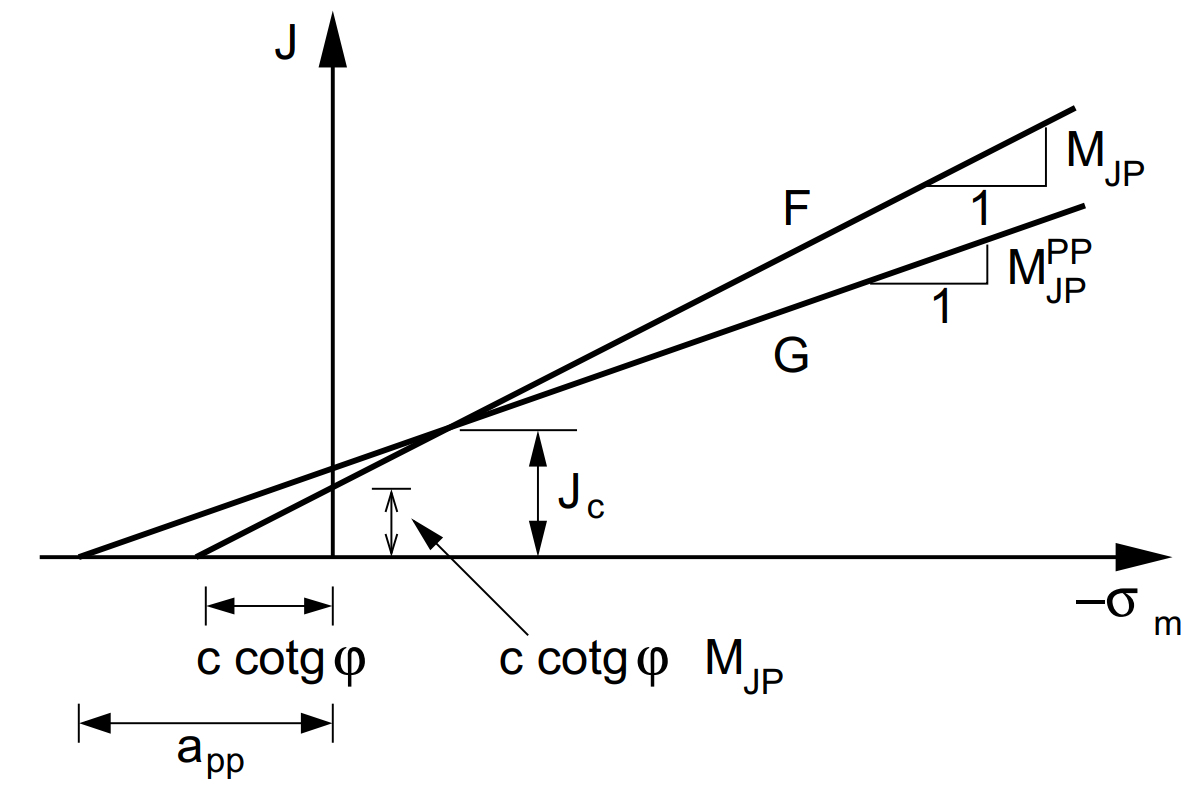
\includegraphics[width=0.7\textwidth, angle=0]{obrazky/drucker_prager_meridian.png}
	\caption[Drucker-Prager yield criterion on meridian plane $T$]{Drucker-Prager yield criterion in meridian plane \cite{geofem}.} \label{obr:M1}
\end{figure}

\subsubsection{Drucker-Prager yield surface}\label{sec:drucker-prager_yield_criterion}
\indent

As written above, Drucker-Prager model extend the von Mises model by including the mean stress in the yield criterion equation, which has the form  

\begin{equation}\label{eq:f_yc}
	F(\sigma) = J + (\sigma_m-c(\kappa_{1}) \cot \varphi(\kappa_{2}) )M_{JP}(\varphi(\kappa_{2})) = 0,
\end{equation}

where $J$ is a square root of the second invariant of the deviatoric stress, $\sigma_m$ is the mean stress with the form 
 
\begin{equation}\label{eq:f_J_sigM}
	J = \sqrt{\dfrac{1}{6} \left[(\sigma_{11}-\sigma_{22})^{2} + (\sigma_{11}-\sigma_{33})^{2} + (\sigma_{22}-\sigma_{33})^{2}\right] + \tau_{12}^{2} + \tau_{13}^{2}+ \tau_{23}^{2}},
\end{equation}


\begin{equation}\label{eq:f_sigM}
	\sigma_m = \dfrac{\sigma_{11} + \sigma_{22} + \sigma_{33}}{3},
\end{equation}

and $M_{JP}$ is used for approximation to the Mohr-Coulomb model and has more forms dependent on point, which approximation is needed. Three different Drucker-Prager cones are in the Fig \ref{obr:F1}. The first one, red circle, touches Mohr-Coulomb yield criterion at $\theta = 30^\circ$ (triaxial compression) with $M_{JP}$ defined as

\begin{figure}[h!]
	\centering	
	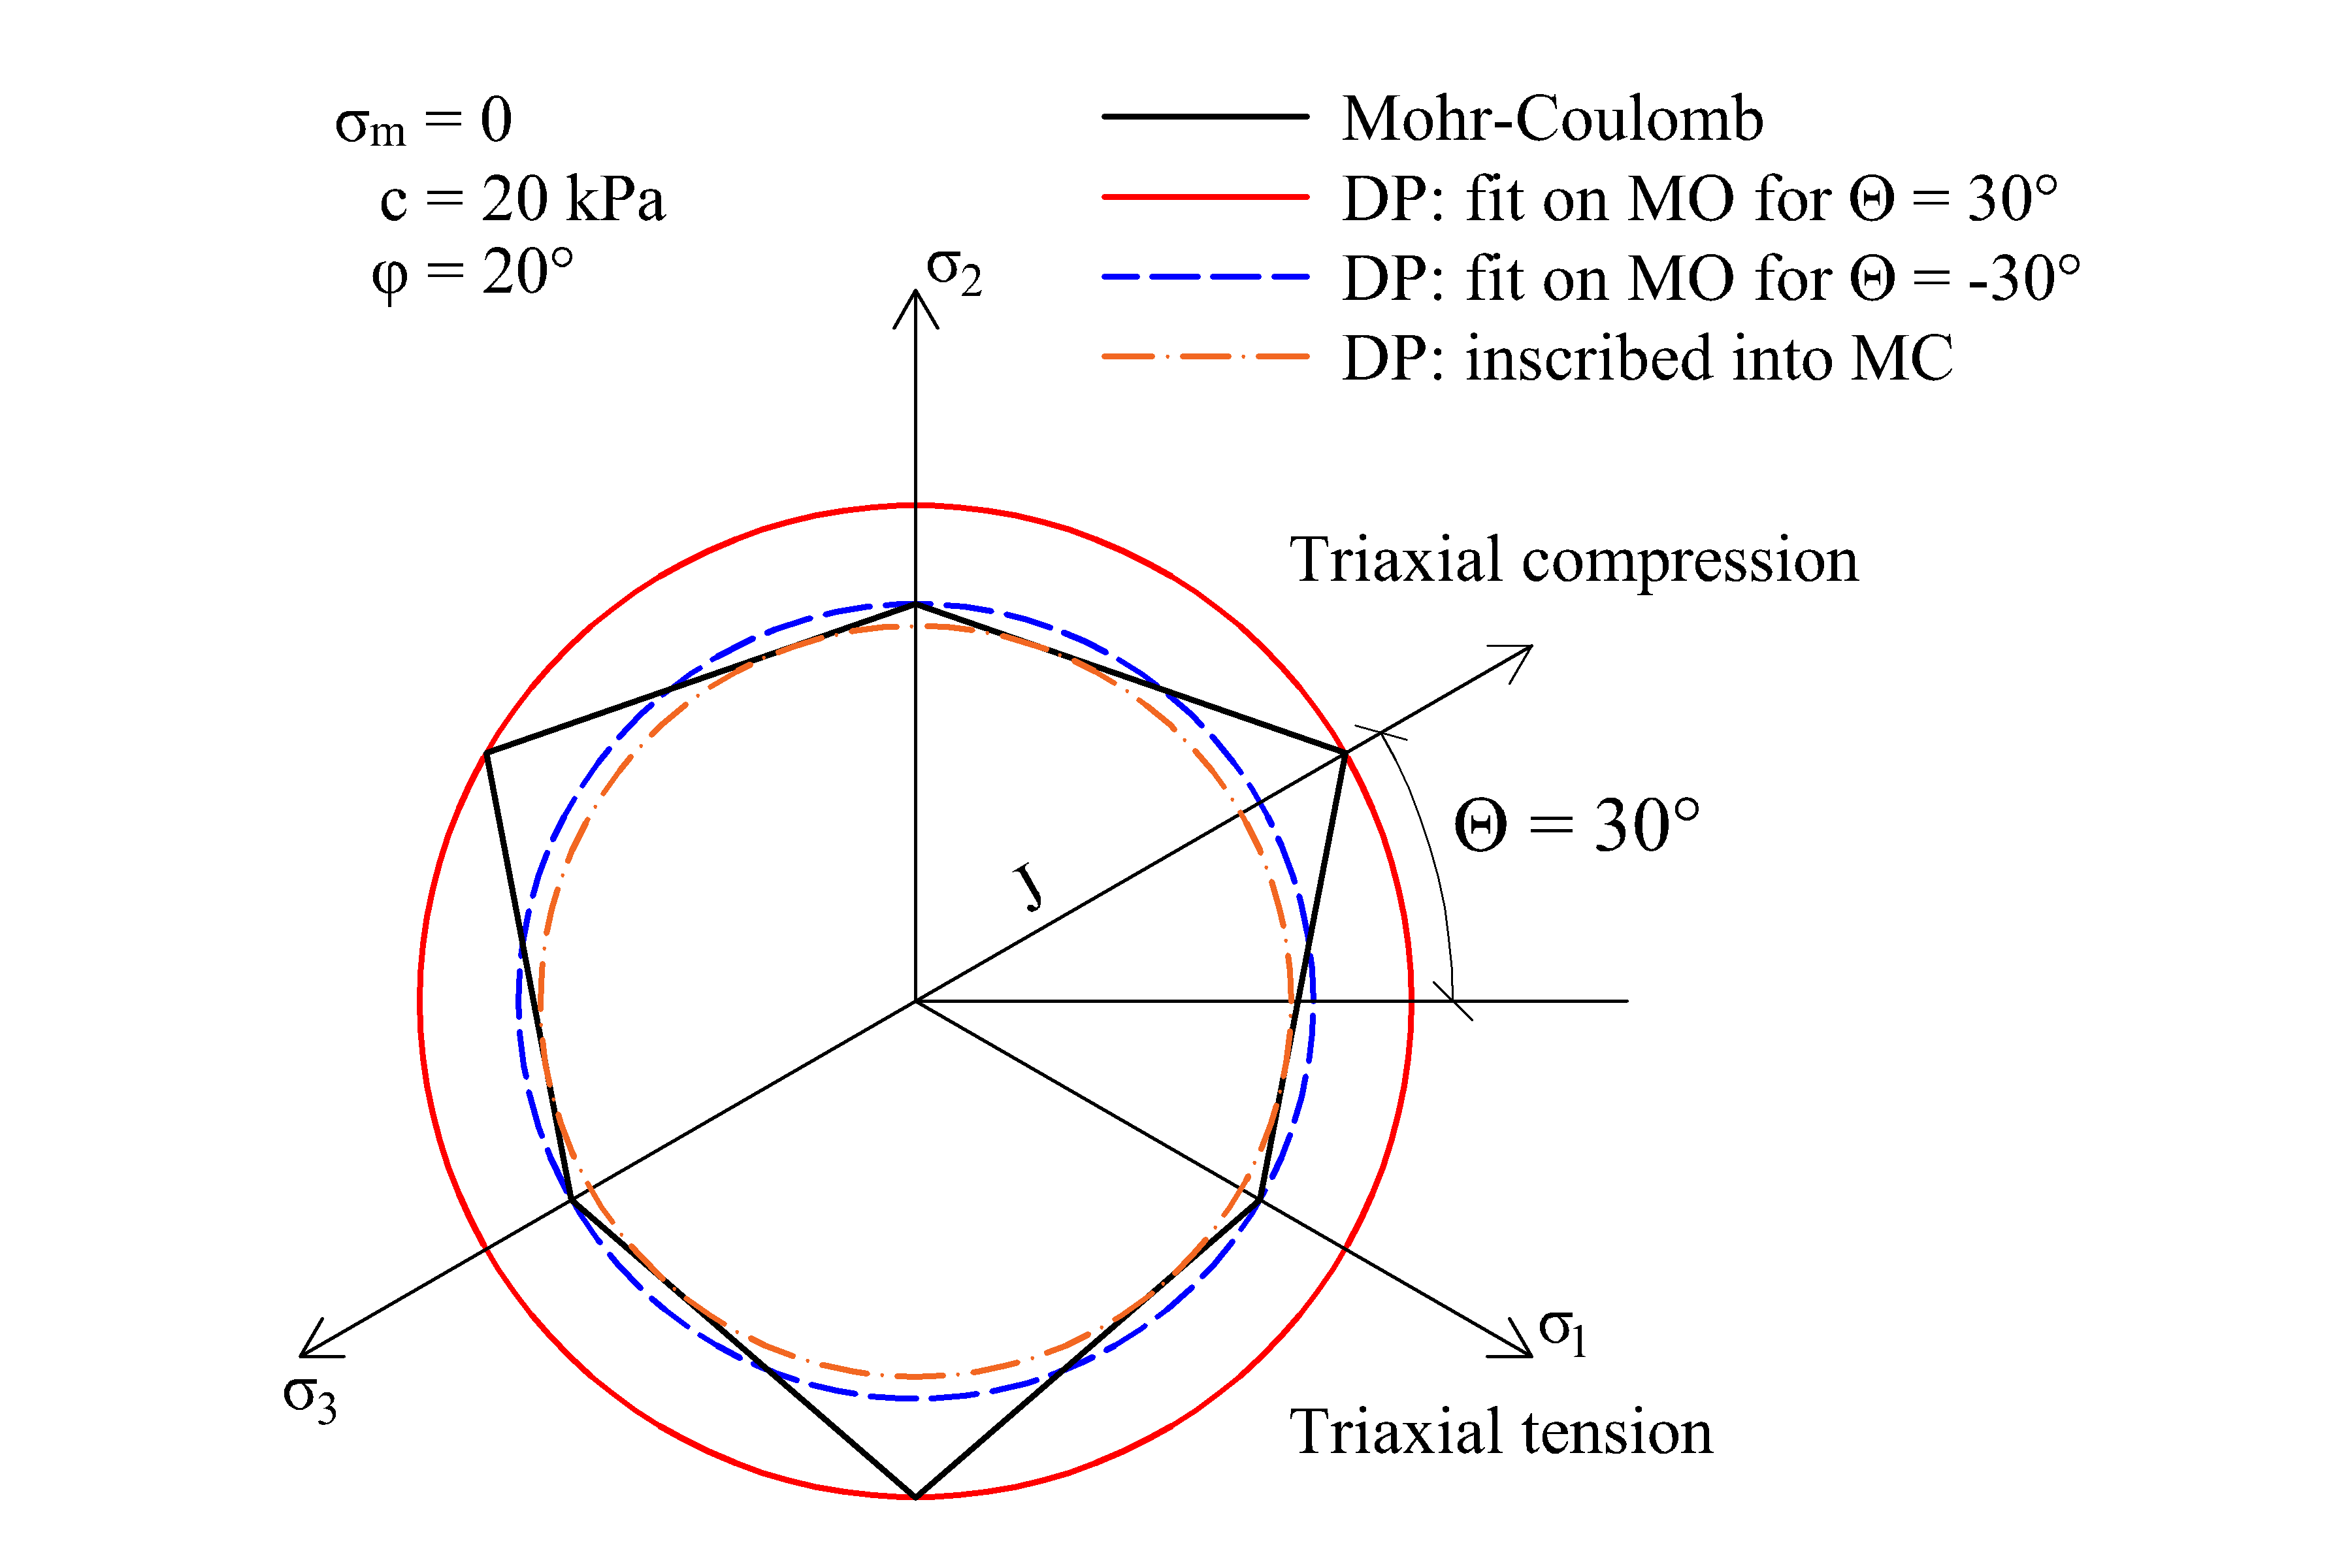
\includegraphics[width=0.8\textwidth, angle=0]{obrazky/drucker-prager_eng.png}
	\caption[Drucker-Prager a Mohr-Coulomb model $T$]{Drucker-Prager and Mohr-Coulomb yield criterion in space of principal stresses. \label{obr:F1}}
\end{figure}



\begin{equation}\label{eq:f_Mjp_30}
	M_{JP}^{\theta=30^\circ} = \dfrac{2\sqrt{3}\sin\varphi}{3-\sin \varphi},
\end{equation}

where $\varphi$ is tangle of internal friction. The second, blue circle, match Mohr-Coulomb model at  $\theta = -30^\circ$ (triaxial tension), can be obtained from

\begin{equation}\label{eq:f_Mjp_-30}
	M_{JP}^{\theta=-30^\circ} = \dfrac{2\sqrt{3}\sin\varphi}{3+\sin \varphi},
\end{equation}

and the last, the green circle is inscribed, and can be determined by

\begin{equation}\label{eq:f_Mjp_i}
	M_{JP} = \dfrac{\sin(\varphi)}{cos(\theta)-\frac{\sin(\theta)\sin(\varphi)}{\sqrt{3}}},
\end{equation}

\begin{equation}\label{eq:f_theta}
	\theta = \arctan{\frac{\sin{\varphi}}{\sqrt{3}}}
\end{equation}

In the Fig \ref{obr:M1} you can see that, Drucker-Prager model is not defined just by the yield function $F$ but also $G$, which is the plastic potential function. $G$ define vector of return to the yield of plasticity, when it is overpassed, and can be written in form 

\begin{equation}\label{eq:G}
	G = J + \left[ \sigma_m - a_{pp} \right] M_{JP}^{PP} = 0,
\end{equation}

where $a_{pp}$ follows from Fig. \ref{obr:M1}. When matching $F$ and $G$ for the current value of stress $\sigma$, result have the form

\begin{equation}\label{eq:app}
	a_{pp} = - \sigma_m^c + ( \sigma_m^c - c\cot\varphi) \dfrac{M_{JP}}{M_{JP}^{PP}}
\end{equation} 

When substituting $a_{pp}$ into the plastic potential function (\ref{eq:G}), it can be rewritten as 

\begin{equation}\label{eq:plastic_potential}
	G = J + \left[ \sigma_m - - \sigma_m + ( \sigma_m^c - c\cot\varphi) \dfrac{M_{JP}}{M_{JP}^{PP}} \right] M_{JP}^{PP} = 0,
\end{equation}

where $M_{JP}^{PP}$ is the gradient of the plastic potential function in $J-\sigma_m$ space (Fig \ref{obr:M1}). When functions of plastic potential and yield function  $M_{JP}^{PP}=M_{JP}$, model becomes associated. $M_{JP}^{PP}$  can be related to the angle of dilatation $\psi$, and can be substituted for $\varphi$ in Equations (\ref{eq:f_Mjp_-30})-(\ref{eq:f_theta}).
 
\subsubsection{Hardening and softening modulus}
\indent

In this model, inspired by the von Mises, is implemented derivation of hardening/softening modulus. To that end, we choose multi-linear form of the hardening/softening law for the cohesion $c$ and the angle of internal friction $\varphi$, as shown in Fig. \ref{obr:H}, where you can also see that, the variation of $c$ and $\varphi$ is a function of deviatoric plastic strain $E_d^{pl}$. Though the components of vector $\kappa$ may vary for each of the two strength parameters, in the present formulation is assumed a single hardening parameter

\begin{equation}\label{eq:kappa}
	\kappa = \kappa_{1} = \kappa_{2} = E_d^{pl}.
\end{equation}

\begin{figure}[h!]
	\centering	
	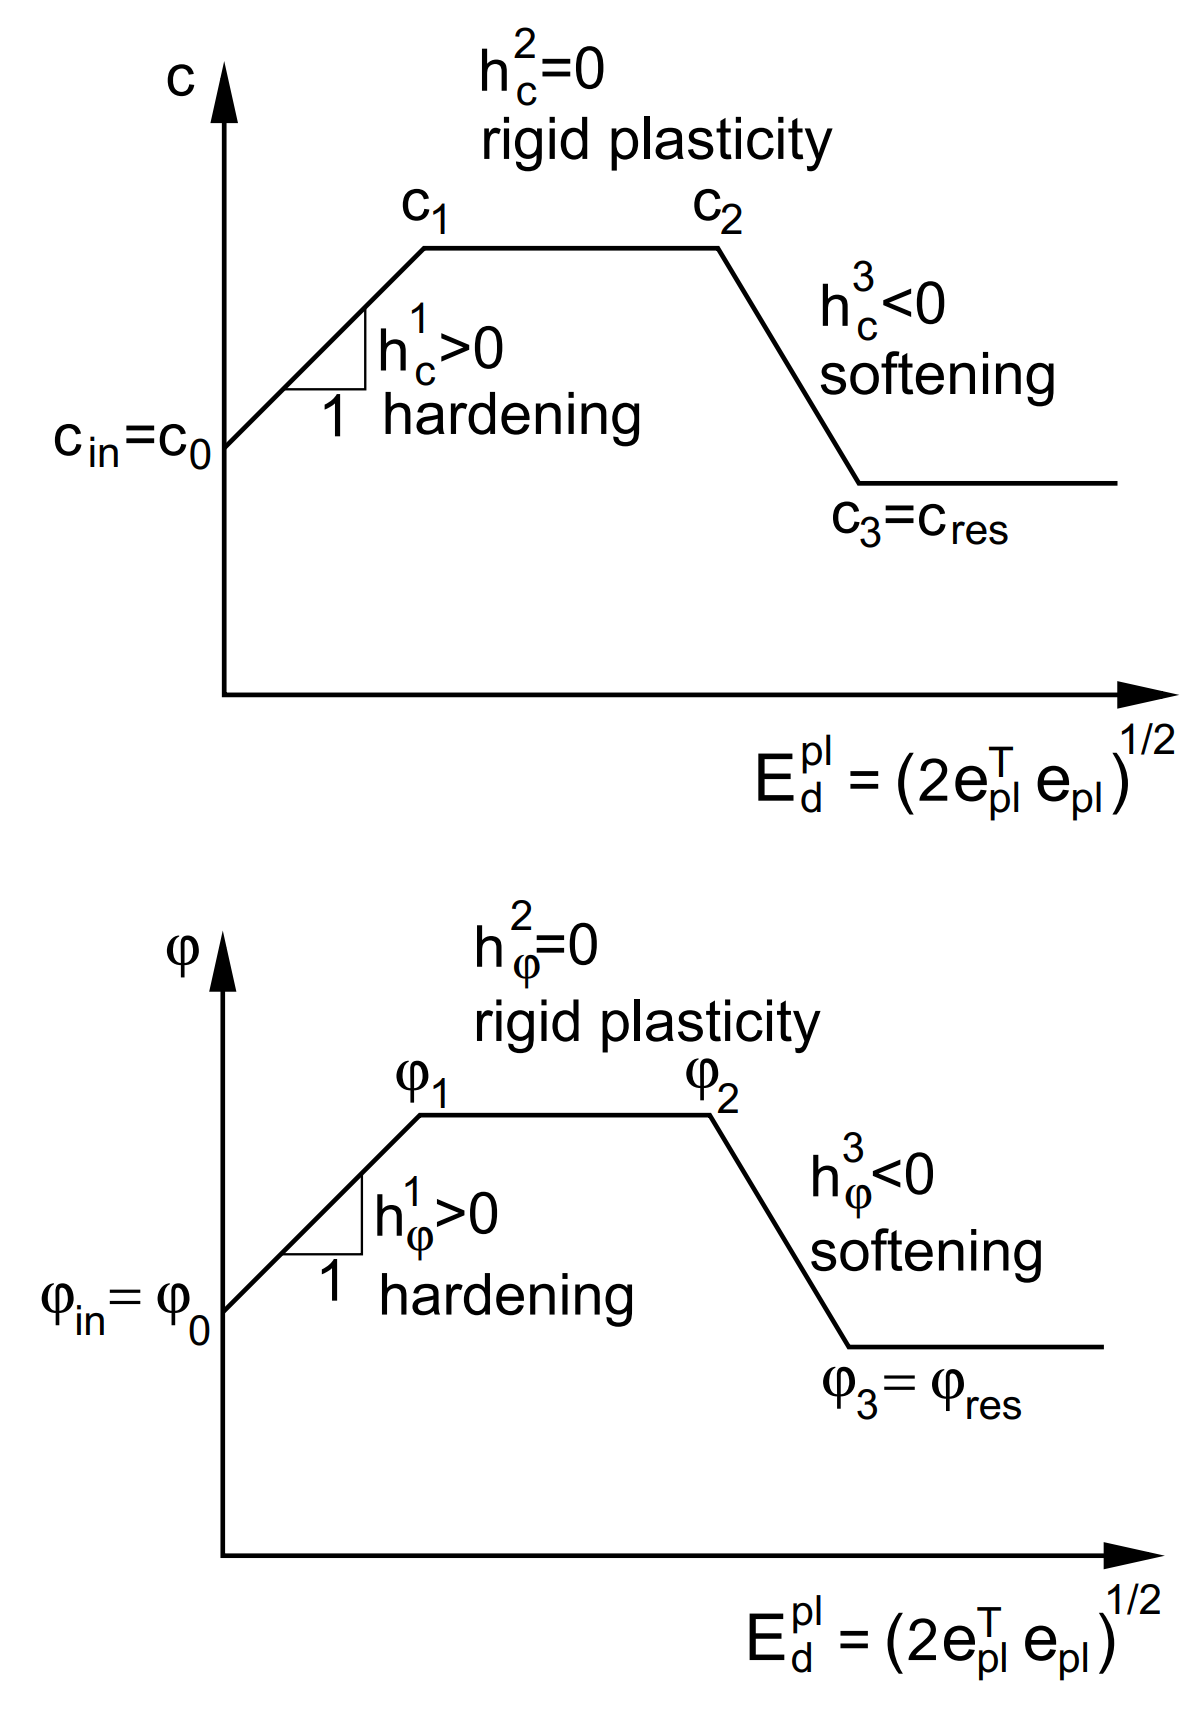
\includegraphics[width=0.8\textwidth, angle=0]{obrazky/hardening_softening_modulus.png}
	\caption[Hardening and softening modulus]{Hardening and softening modulus \cite{geofem}: $c_{in}$ and $c_{res}$, respective $\varphi_{in}$ and $\varphi_{res}$ represent initial and residual values of $c$ and $\varphi$.} \label{obr:H}
\end{figure}
 
Multi-linear formulation suppose that and $n^{th}$ interval in the Fig. \ref{obr:H} is active, then the current strenght parameters can be provided by

\begin{equation}\label{eq:c}
	c = c^{n-1} + h_c^n \left( E_d^{pl} -(E_d^{pl})^{n-1} \right),
\end{equation}

\begin{equation}\label{eq:phi}
\varphi = \varphi^{n-1} + h_\varphi^n\left( E_d^{pl} - (E_d^{pl})^{n-1} \right),
\end{equation}

where $h_c^n$ and $h_\varphi^n$ are the hardening/softening moduli for $c$ and $\varphi$ and can be written in the form


\begin{equation}\label{eq:h_c}
	h_c^n = \dfrac{c^n-c^{n-1}}{(E_d^{pl})^{n}-(E_d^{pl})^{n-1}}
\end{equation}

\begin{equation}\label{eq:h_phi}
 	\varphi_c^n = \dfrac{\varphi^n-\varphi^{n-1}}{(E_d^{pl})^{n}-(E_d^{pl})^{n-1}}
\end{equation}

From \cite{geofem} hardening modulus can be determined by

\begin{equation}\label{eq:H_first}
	H = \left(-\dfrac{\partial F}{\partial \kappa}\right)^T \dfrac{\partial \kappa}{\partial \lambda},
\end{equation}
\newpage
and referring to Fig. \ref{obr:H} and using Eq. (\ref{eq:H_first}) the hardening/softening modulus $H$ assumes the form 

\begin{equation}\label{eq:H}
	H = - \pdv{F}{c} \dv{c}{E_d^{pl}} \dv{E_d^{pl}}{\lambda} - \pdv{F}{\varphi} \dv{\varphi}{E_d^{pl}} \dv{E_d^{pl}}{\lambda},
\end{equation}

where
\begin{align}
\pdv{F}{\varphi}& = \dfrac{c}{\sin^2\varphi} M_{JP} + (\sigma_m - c\cot \varphi) \dv{M_{JP}}{\varphi},\label{eq:F/phi}\\
\dv{F}{c}& = - \cot \varphi M_{JP},\\
\dv{c}{\kappa}& = \dv{c}{E_d^{pl}} = h_c,\\
\dv{\varphi}{\kappa}& = \dv{\varphi}{E_d^{pl}} = h_\varphi
\end{align}

Partial derivations of $M_{JP}$ with respect to $\varphi$ for selected values of $\theta$ are

\begin{align}
	\dv{M_{JP}^{ins}}{\varphi}					& = \dfrac{3\sqrt{3}\cos \varphi}{(3 + \sin^2 \varphi)^{\frac{3}{2}}},\\
	\dv{M_{JP}^{\theta = \ang{-30}}}{\varphi}	& = \dfrac{6\sqrt{3}\cos \varphi}{(1-\sin \varphi)^2},\\
	\dv{M_{JP}^{\theta = \ang{30}}}{\varphi}	& = \dfrac{6\sqrt{3}\cos \varphi}{(1+\sin \varphi)^2}.
\end{align}


When we accept the strain hardening approach, then we can write

\begin{align}
	\dd\varepsilon^{pl}& = \dd\lambda\pdv{G}{\sigma} = \dd\lambda\dfrac{1}{2J}P\sigma,\\
	\dd\kappa& = \dd E_d^{pl} = \sqrt{2(\varepsilon^{pl})^T \text{\textbf{QPQ}} \varepsilon^{pl} } = \dd \lambda = \dv{E_d^{pl}}{\lambda} = 1.\label{eq:dkappa}
\end{align}

With final substitution of Eq. (\ref{eq:F/phi})-(\ref{eq:dkappa}) back into Eq. (\ref{eq:H}), result is searched form of the hardening/softening modulus as

\begin{equation}\label{eq:H_final}
	H = h_c \cot\varphi M_{JP} - h_\varphi \left[ \dfrac{c}{\sin^2 \varphi} M_{JP} + (\sigma_m - c \cot \varphi) \dv{M_{JP}}{\varphi} \right].
\end{equation}


\subsubsection{Calculation procedure and implementation}\label{sec:drucker-prager_count}
\indent

Total elastic stress can be calculated as 
\begin{equation}\label{eq:f_sigma}
\sigma = \text{\textbf{D}}^{el} \varepsilon_{el},
\end{equation}
where \textbf{D}$^{el}$ is ordinary stiffness matrix and $\varepsilon_e$ is elastic deformation. Calculation is performed in  implicit software \cite{mars}, so model is implemented with increments. Then can be equation modified as

\begin{equation}\label{eq:f_sigma1}
	\sigma^{n+1} = \sigma^n+ \text{\textbf{D}}^{el} \mathrm{d} \varepsilon_{el}.
\end{equation}

Next step in calculation is determine, if is Eq. (\ref{eq:f_yc}) satisfied, if is, strains ans stresses are stored, and calculation continues with next deformation increment. If yield function exceeded, material behavior become to be from basic elastic to elasto-plastic with hardening. Due to higher amount of the variables, which describe return to the yield of plasticity, is necessary to implement the Jacobian matrix\footnote{Matrix of partial derivations}. There are four material parameters that may be calculated, when is performed return to yield of plasticity:

\begin{itemize}
	\item $\Delta\lambda$ - Coefficient of plastic flow,
	\item $c$ - Cohesion,
	\item  $\varphi$ - Angle of friction,
	\item $\psi$ - Angle of dilatation.
\end{itemize}

Before of describing Jacobian matrix, we need to find out basic equations, which are used in it and define dependence of all variables. 
Plastic strain increment have the form 

\begin{equation}
	\dd \varepsilon^{pl} = \Delta \lambda \pdv{G}{\sigma},
\end{equation}

and with accepting this flow rule, increments of yield respective plastic strain have the form 

\begin{align}
	\dd \varepsilon_\nu^{pl} &= \dd \lambda \pdv{G}{\sigma_m} = \Delta \lambda M_{JP}^{PP} \sin \psi,\\
	%\dd e^{pl} &= \dd \lambda \pdv{G}{s} = \dd \lambda \dfrac{\text{\textbf{G}}^{-1}s}{2J}\text{ where } s = \text{\textbf{PQ}}\sigma,\\
	\dd E_{d}^{pl} &= \dd \lambda \pdv{G}{J} = \Delta \lambda,
\end{align}

which further allows writing the corresponding stresses at the end of the $i+1$ load increment as  

\begin{align}
	\sigma_m^{i+1} &= \sigma_m^{tr} - K M_{JP}^{PP} (\sin \psi^{i+1}) \Delta \lambda,\\
	%s^{i+1} &= s^{tr} - 2\mu \Delta \lambda\dfrac{s^{i+1}}{2J^{i+1}} = \dfrac{s^{tr}}{1 + \dfrac{\mu \Delta \lambda}{J^{i+1}}} = s^{tr} \left( 1 - \dfrac{\mu \Delta \lambda}{J^{tr}}   \right),\\
	J^{i+1} &= J^{tr} + \mu \Delta \lambda,
\end{align}

where $K$ is the bulk modulus and $\mu$ represent the elastic shear modulus to avoid misinterpretation with the plastic potential function. Now can be the Jacobian matrix defined.

\begin{itemize}
	\item Primary variables
	
	\begin{equation}
		\lbrace \mathbf{a} \rbrace ^T = \lbrace \Delta \lambda, c^{i+1}, \varphi^{i+1}, \psi^{i+1} \rbrace.
	\end{equation}
	
	\item Residuals
	\begin{equation}
		\lbrace \mathcal{r} \rbrace =  \lbrace \mathcal{F}, \mathcal{C}, \mathrm{\Phi}, \mathrm{\Psi} \rbrace,
	\end{equation}
	where \begin{align}
		\mathcal{F} &= \overbrace{J^{tr}-\mu\Delta\lambda}^{J^{i+1}} + [\overbrace{\sigma_m^{tr}-K M_{JP}^{PP}(\sin \psi^{i+1})\Delta\lambda}^{\sigma_m^{i+1}}-c^{i+1}\cot\varphi^{i+1}]M_{JP}(\sin\varphi^{i+1}),\label{eq:f_yc_lam}\\
		\mathcal{C} &= c^{i+1} - \hat{c} = 0,\label{eq:C_jac}\\
		\mathrm{\Phi} &= \varphi^{i+1} - \hat{\varphi} = 0,\label{eq:phi_jac}\\
		\mathrm{\Psi} &= \psi^{i+1} - \hat{\psi} = 0.
	\end{align}
	Variables $\hat{c}$ and $\hat{\varphi}$ follows Eq.(\ref{eq:c}) and (\ref{eq:phi}) and the current value of dilatation angle $\hat{\psi}$ can be, with help of Rowe's dilatation theory in triaxial compression, written as
	\begin{equation}
		\sin \hat{\psi} = \dfrac{\sin \varphi^{i+1} - \sin \varphi_{cv}}{1_- \sin \varphi^{i+1} \sin \varphi_{cv}},
	\end{equation}
	where $\varphi_{cv}$ is constant-volume friction angle.
	
	\item Local Newton-Raphson method
	\begin{equation}\label{eq:newton_raphson}
		\lbrace a^{i+1} \rbrace _{k+1} = \lbrace a^{i+1}_k \rbrace - [\text{\textbf{H}}]^{-1} \lbrace r \rbrace_k 
	\end{equation}
	
	\item Jacobian matrix $[\textbf{H}]$
	\begin{equation}
		[\text{\textbf{H}}] = \mqty[\pdv{J}{\Delta \lambda} \pdv{\mathcal{F}}{\sigma_m} \pdv{\sigma_m}{\Delta \lambda} & \pdv{\mathcal{F}}{c} & \pdv{\mathcal{F}}{\varphi} + \pdv{\mathcal{F}}{M_{JP}} \pdv{M_{JP}}{\sin \varphi} & \pdv{\mathcal{F}}{M_{JP}^{PP}} \pdv{M_{JP}^{PP}}{\sin \psi}\\
		\pdv{\mathcal{C}}{\hat{c}} = \pdv{\hat{c}}{\Delta \lambda} & \pdv{\mathcal{C}}{c} & 0 & 0\\
		\pdv{\mathrm{\Phi}}{\sin \hat{\varphi}} = \pdv{\hat{\varphi}}{\Delta \lambda} & 0 & \pdv{\mathrm{\Phi}}{\sin \varphi} & 0 \\
		0 & 0 & \pdv{\mathrm{\Psi}}{\sin \hat{\psi}} \pdv{\sin \hat{\psi}}{\sin \varphi} & \pdv{\mathrm{\Psi}}{\sin \psi}]
	\end{equation}
	where partial derivations are
	
	\begin{align}
		&\pdv{J}{\Delta \lambda} \pdv{\mathcal{F}}{\sigma_m} \pdv{\sigma_m}{\Delta \lambda}  = -\mu - K M_{JP}^{PP}M_{JP},\\
		&\pdv{\mathcal{F}}{c} = -M_{JP}\tan\varphi,\\
		&\pdv{\mathcal{F}}{\varphi} + \pdv{\mathcal{F}}{M_{JP}} \pdv{M_{JP}}{\sin \varphi} = M_{JP} \dfrac{c}{\sin^2\varphi \cos\varphi} + \left( \sigma_m \dfrac{c}{\tan \varphi} \right) \dv{M_{JP}}{\sin \varphi}, \\
		&\pdv{\mathcal{F}}{M_{JP}^{PP}} \pdv{M_{JP}^{PP}}{\sin \psi} = -K \Delta \lambda \dv{M_{JP}^{PP}}{\sin \psi},\\
		&\pdv{\mathcal{C}}{\hat{c}} = \pdv{\hat{c}}{\Delta \lambda} = -h_c, \\
		&\pdv{\mathcal{C}}{c} = 1,\\
		&\pdv{\mathrm{\Phi}}{\sin \hat{\varphi}} = \pdv{\hat{\varphi}}{\Delta \lambda} = -\cos(\varphi) h_{\varphi},\\
		&\pdv{\mathrm{\Phi}}{\sin \varphi} = 1,\\
		&\pdv{\mathrm{\Psi}}{\sin \hat{\psi}} \pdv{\sin \hat{\psi}}{\sin \varphi} = -\dfrac{1 - \sin^2\varphi_{cv} }{1-\sin \varphi \sin \varphi_{cv}},\\
		&\pdv{\mathrm{\Psi}}{\sin \psi} = 1.
	\end{align}
	
	Derivation of $M_{JP}$ with respect to $\sin \varphi$ is not writed in exact form due to variable equation of $M_{JP}$ (\ref{eq:f_Mjp_30})-(\ref{eq:f_Mjp_i}).
	
	\item Initial conditions
	
	\begin{align}
		\lbrace a_0 \rbrace^T &= \lbrace 0, c^i, \sin \varphi^i, \sin \psi^i \rbrace,\\
		\lbrace r_0 \rbrace^T &= \lbrace J^{tr} + (\sigma_m^{tr}-c^i\cot\varphi^i)M_{JP}(\sin\varphi^i), 0, 0, 0 \rbrace.
	\end{align}
	
\end{itemize} 

\subsubsection{Apex problem}
\indent

In the Fig \ref{obr:apex_cones} you can see two cones. First $K_\varepsilon$ (following direction of the plastic strain vector), which shows inadmissible region for the plastic strain increment, and $K_\sigma$, which show the admissible stress domain. Its obvious that, if is standard stress point in region $K_\sigma$, material behaviors is elastic, when it is outside of $K_\sigma$ but also outside of $K_\varepsilon$, computation is performing regular stress return. But the non-associated flow rule restrict the plastic strain increment to belong in the cone $K_\varepsilon$ (Eq. \ref{eq:eps_apex}), so if it belongs, stress should be returned to the apex point. That situation may occur in two cases (Fig. \ref{obr:apex_return}): $(a)$ right after load increment, bud also $(b)$, when performing regular stress return, due change of material parameters. Such a situation can be referred as an "apex problem". 

\begin{equation}\label{eq:eps_apex}
	\dot{\varepsilon}_v \geq M_{JP}^{PP} \dot{E}_d^{pl}.
\end{equation}

In the literature we can find two different stands for performing apex problem:

\begin{itemize}
	\item Return with constant material parameters.
	\item Return with hardening/softening material.
\end{itemize}
At the first case, stress point just return to the apex (Fig.\ref{obr:apex_cones}), so stress form is

\begin{equation}\label{eq:sigPL}
	\sigma^{i+1} = 3c^{i} \cot \varphi^{i} \textbf{m}.
\end{equation}

In \cite{geofem} author show a variational form of the flow rule to show through the concept of bi-potentials that the vector of plastic strain increments for the apex problem is provided by

\begin{equation}\label{eq:epsPL}
	\Delta\varepsilon^{pl} = (\textbf{D})^{-1}( \sigma^{tr} - 3 c^{i+1} \cot \varphi^{i+1} \textbf{m} )
\end{equation}

under condition



\begin{equation}\label{eq:flow_condition}
\dfrac{1}{G} M_{JP}^{PP} J^{tr} - \dfrac{1}{K} (\sigma_m^{tr} - c^i \cot \varphi^i) < 0.
\end{equation}

Note that Eq. (\ref{eq:flow_condition}) is essentially linearized from of a Eq. (\ref{eq:sigPL}).

\begin{figure}[h!]
	\centering	
	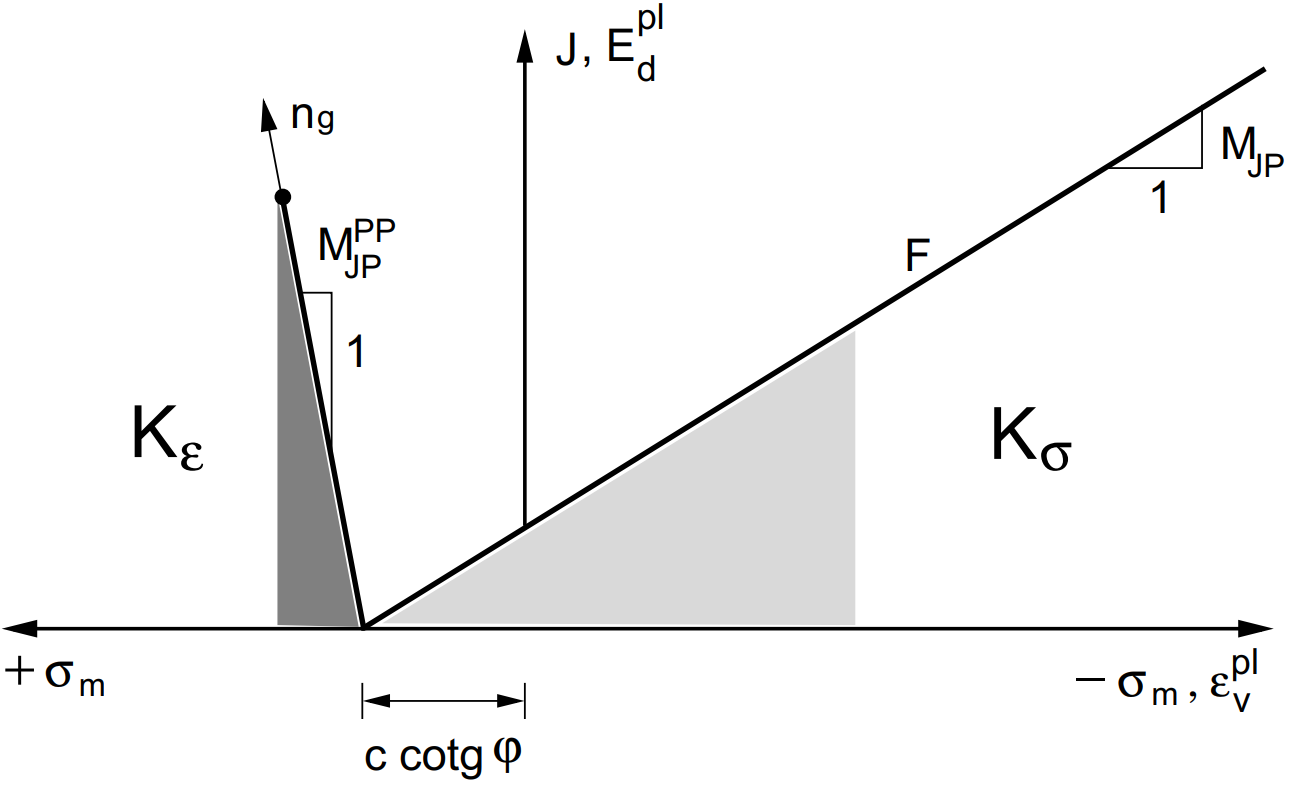
\includegraphics[width=0.8\textwidth, angle=0]{obrazky/apex_cones.png}
	\caption[Apex abmissible regions]{Apex admissible regions for stresses and plastic strain rates \cite{geofem}.} \label{obr:apex_cones}
\end{figure}


\begin{figure}[h!]
	\centering	
	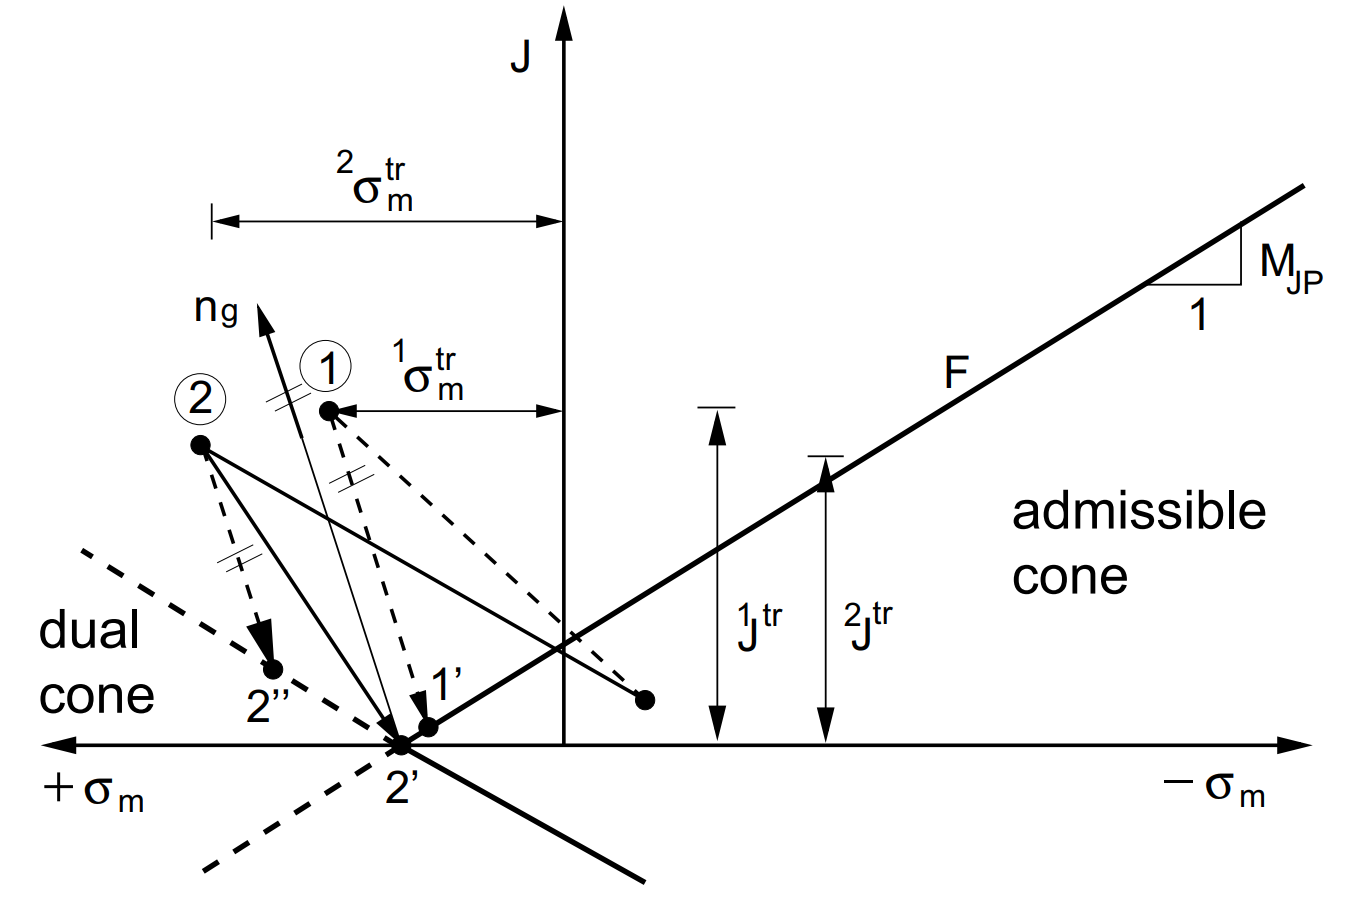
\includegraphics[width=0.8\textwidth, angle=0]{obrazky/apex_recursive_return.png}
	\caption[Apex return]{Apex regular and singular return \cite{geofem}: .} \label{obr:apex_return}
\end{figure}


If we choose second approach of assuming hardening/softening material, we need to update $c$ and $\varphi$ with apex return. Procedure is similar to the regular plasticity return, but with different equations. Before proceeding, we recall that the strain hardening hypotheses is adopted with a single hardening/softening parameter $\kappa$ with form

\begin{equation}\label{eq:hardening_parameter}
	\dot{\kappa} = \dot{E}_d^{pl}
\end{equation}

With Eq. \ref{eq:hardening_parameter} we can reach incremental nonlinear equation with form

\begin{equation}
	\mathcal{E} = \Delta E_d^{pl} - \overbrace{\sqrt{2(\Delta \varepsilon^{pl})^T \textbf{QPQ}\Delta\varepsilon^{pl}} }^{\Delta \hat{E}_d^{pl}}=0
\end{equation}

which would be solved simultaneously with Eq.(\ref{eq:C_jac}) and (\ref{eq:phi_jac}). Note that the increment of plastic strain given by Eq. (\ref{eq:epsPL}) is a function of current strength parameters

\begin{equation}
	\Delta\varepsilon^{pl} = \Delta\varepsilon^{pl} (c^{i+1}, \varphi^{i+1}).
\end{equation}

Due to analogy with the regular return to the yield surface we can also use Newton-Raphson method (Eq.(\ref{eq:newton_raphson})). The calculation procedure is defined:

\begin{itemize}
	\item Primary variables
	
	\begin{equation}
		\lbrace a \rbrace^T = \lbrace \Delta E_d^{pl}, c^{i+1}, \varphi^{i+1} \rbrace.
	\end{equation}
	
	\item Residuals
	
	\begin{equation}
		\lbrace r \rbrace ^T = \lbrace \mathcal{E}, \mathcal{C}, \mathrm{\Phi} \rbrace
	\end{equation}
	
	\item Jacobian Matrix [\textbf{H}]
	
	\begin{equation}
		[\text{\textbf{H}}] = \mqty[\pdv{\mathcal{E}}{\Delta E_d^{pl}} & \pdv{\mathcal{E}}{\Delta\varepsilon^{pl}}^T \pdv{\Delta\varepsilon^{pl}}{c} & \pdv{\mathcal{E}}{\Delta\varepsilon^{pl}}^T \pdv{\Delta\varepsilon^{pl}}{\sin \varphi}\\
		\pdv{\mathcal{C}}{\Delta E_d^{pl}} = \pdv{\mathcal{C}}{\Delta \lambda} & \pdv{\mathcal{C}}{c} & 0 \\
		\pdv{\mathrm{\Phi}}{\Delta E_d^{pl}} = \pdv{\mathrm{\Phi}}{\Delta \lambda} & 0 & \pdv{\mathrm{\Phi}}{\sin \varphi}]
	\end{equation}
	\newpage
	where partial derivations have the form\
	
	\begin{align}
		&\pdv{\mathcal{E}}{\Delta E_d^{pl}} = 1,\\
		&\pdv{\mathcal{E}}{\Delta\varepsilon^{pl}}^T \pdv{\Delta\varepsilon^{pl}}{c} =  -\dfrac{2}{\Delta E_d^{pl}} \Delta e_{pl}^T (-3\cos\varphi^{i+1}\textbf{m}) = \dfrac{6\cos\varphi^{i+1}}{ \Delta E_d^{pl}} \Delta e_{pl}^T \textbf{m},\\
		&\pdv{\mathcal{E}}{\Delta\varepsilon^{pl}}^T \pdv{\Delta\varepsilon^{pl}}{\sin \varphi} = \pdv{\Delta\varepsilon^{pl}}{c} =  -\dfrac{2}{ \Delta E_d^{pl}} \Delta e_{pl}^T (-3c^{i+1}\textbf{m}) = \dfrac{6 c^{i+1}}{ 
		 \Delta	E_d^{pl}} \Delta e_{pl}^T \textbf{m} ,\\
		&\pdv{\mathcal{C}}{\Delta E_d^{pl}} = \pdv{\mathcal{C}}{\Delta \lambda} =  -h_c,\\
		&\pdv{\mathcal{C}}{c} = 1,\\
		&\pdv{\mathrm{\Phi}}{\Delta E_d^{pl}} = \pdv{\mathrm{\Phi}}{\Delta \lambda} = -\cos(\varphi) h_{\varphi} ,\\
		&\pdv{\mathrm{\Phi}}{\sin \varphi} = 1.
	\end{align}
	
	where $e_{pl}$ is deviatoric part of plastic strain tensor. 
		
	\item Initial conditions
	\begin{equation}
		\lbrace a_0 \rbrace^T = \lbrace 0, c^i, \varphi^i\rbrace,
	\end{equation}
	
	\begin{equation}
		\lbrace r_0 \rbrace^T = \lbrace \sqrt{2(\Delta \varepsilon^{pl})^T(c^i, \varphi^i) \textbf{QPQ}\Delta\varepsilon^{pl}(c^i, \varphi^i)}, 0, 0\rbrace.
	\end{equation}
\end{itemize}
 
